\documentclass{article}[18pt]
\usepackage[utf8]{inputenc}
\usepackage[margin=0.7in]{geometry}
\usepackage{parselines} 
\usepackage{amsmath}
\usepackage{titlesec}
\usepackage{pgfplots}
\usepackage{graphicx}
\usepackage{tabularx}
\usepackage[english]{babel}
\usepackage{fancyhdr}
\usepackage{circuitikz}
\pgfplotsset{width=10cm,compat=1.9}
\usepackage{relsize}
\titlespacing\section{0pt}{14pt plus 4pt minus 2pt}{0pt plus 2pt minus 2pt}
\newlength\tindent
\setlength{\tindent}{\parindent}
\setlength{\parindent}{0pt}
\renewcommand{\indent}{\hspace*{\tindent}}

\pagestyle{fancy}
\fancyhf{}
\rhead{Sam Robbins 13SE}
\lhead{AS Level Physics - Mechanics and Materials}
\rfoot{Page \thepage}


\begin{document}
\begin{center}
\underline{\huge Materials}
\end{center}
\section{Bulk Properties of solids}
\textbf{Hooke's law} - Force is directly proportional to extension, provided the proportionality limit has not been reached
\subsection{Spring constant}
\subsubsection{Series}
$$\text{Spring constant}=\dfrac{\text{Spring constant of one spring}}{\text{Number of springs}}$$
\subsubsection{Parallel}
$$\text{Spring constant=Spring constant of one spring} \times \text{Number of springs}$$
\subsection{Material properties}
\textbf{Brittle material} - Snap\\
\textbf{Ductile material} - Stretch\\
\textbf{Plastic Behaviour} - The behaviour of a material after it has reached it's elastic limit
\subsection{Stress strain graph of a metal wire}
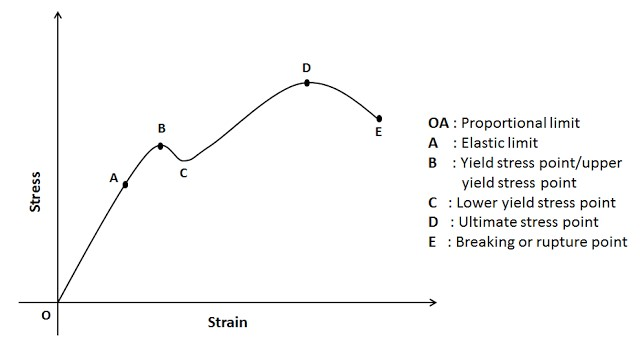
\includegraphics[width=4in]{Stress_Strain.jpg}\\
\section{The Young Modulus}
The \textbf{gradient}of a stress strain graph is the Young Modulus\\
\\
\textbf{Units} of Young Modulus: $\text{Nm}^{-2}$ or Pa\\
\\
\textbf{Stiff Material} - \textbf{High} Young Modulus\\
\textbf{Flexible Material} - \textbf{Low} Young Modulus\\
\newpage
\subsection{Searle's apparatus for measuring Young's Modulus}
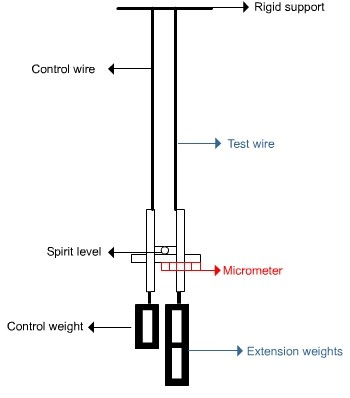
\includegraphics[width=3in]{Searle.jpg}\\
\subsection{Vernier apparatus for measuring Young's Modulus}
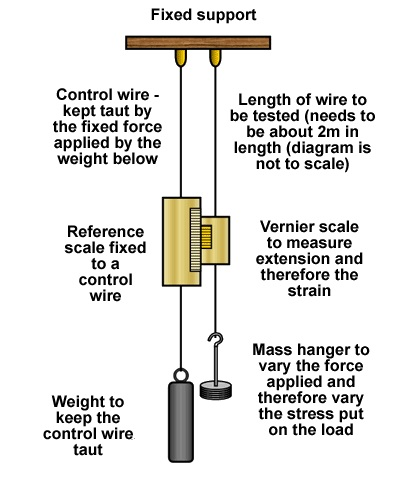
\includegraphics[width=3in]{young_modulus.jpg}\\
\newpage
\section{Stress Strain Graphs}
\subsection{Rubber}
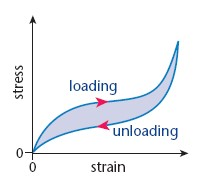
\includegraphics[width=2in]{rubber.jpg}\\
\subsection{Metal}
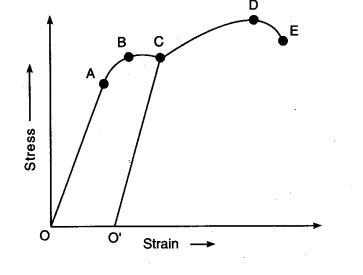
\includegraphics[width=2in]{metal.jpg}\\
\subsection{Polythene}
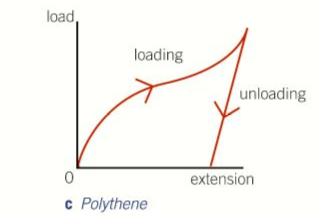
\includegraphics[width=2in]{Polythene.png}\\
\end{document}
